%------------------------------------------------------------
% DEFINITIONS AND HEADERS -- IGNORE THIS
%------------------------------------------------------------
\documentclass{article}
\usepackage[top=2.2cm, bottom=2.1cm, left=2.2cm, right=2.2cm]{geometry}
\usepackage[utf8]{inputenc}
\usepackage{algpseudocode}
% Get better typography
\usepackage[protrusion=true,expansion=true]{microtype}  
% For algorithms
\usepackage[boxruled,linesnumbered,vlined,inoutnumbered]{algorithm2e}
\SetKwInOut{Parameter}{Parameters}
% For basic math, align, fonts, etc.
\usepackage{amsmath}
\usepackage{amsthm}
\usepackage{amssymb}
\usepackage{longtable}
\usepackage{listings}
\lstset{
    basicstyle=\ttfamily,
    breaklines=true,
    columns=flexible
}

\usepackage{mathtools}
\usepackage{mathrsfs}
\usepackage{rotating}
\usepackage{tabularx}
\usepackage{fvextra}
\usepackage{booktabs}
\usepackage{soul}
\usepackage{changepage}
\usepackage{gensymb} % For \degree
\usepackage{lscape}
% For \thead to make line breaks in tables
\usepackage{array}
\usepackage{makecell}
\renewcommand\theadalign{bc}
\renewcommand\theadfont{\bfseries}
\renewcommand\theadgape{\Gape[4pt]}
\renewcommand\cellgape{\Gape[4pt]}
\usepackage{courier} % For \texttt{foo} to put foo in Courier (for code / variables)
\usepackage{lipsum} % For dummy text
% For images
\usepackage{graphicx}
\usepackage{subcaption}
\usepackage[space]{grffile} % For spaces in image names
% For bibliography
\usepackage[round]{natbib}
% For color
\usepackage{xcolor}
\definecolor{light-grey}{rgb}{0.9,0.9,0.9}
\definecolor{dark-red}{rgb}{0.4,0.15,0.15}
\definecolor{dark-blue}{rgb}{0,0,0.7}
\definecolor{darkblue}{rgb}{0,0,.6}
\definecolor{darkred}{rgb}{.58,0,0}
\definecolor{brighterred}{rgb}{.745,0,0}
\definecolor{darkgreen}{rgb}{0,.6,0}
\definecolor{red}{rgb}{.98,0,0}
\usepackage{environ}
% Only show sections in table of contents and rename
\setcounter{tocdepth}{2}
\renewcommand{\contentsname}{Table of Contents}
% For links (e.g., clicking a reference takes you to the phy)
\usepackage{hyperref}
\hypersetup{
    colorlinks, linkcolor={dark-blue},
    citecolor={dark-blue}, urlcolor={dark-blue}
}
\newcommand{\HIGHLIGHT}[1]{\textcolor{blue}{\textbf{#1}}}
% \newcommand{\Solution}[1]{{\color{blue} \paragraph{\bf $\bigstar $ SOLUTION:} { \sf
%     #1} \bigskip}}
\newcommand{\TODO}[1]{\textcolor{blue}{\textbf{{#1}}}}
\newcommand{\POINTS}[1]{\textcolor{purple}{\textbf{{#1}}}}
\providecommand{\mathcolor}[2]{\textcolor{#1}{#2}}
% My definition of "summary boxes" (see below)
\usepackage[most]{tcolorbox}
\definecolor{boxgray}{rgb}{0.95, 0.95, 0.95}
\definecolor{boxblue}{rgb}{0.941, 0.941, 0.98}
\definecolor{boxpink}{rgb}{1.0, 0.93, 0.93}
\definecolor{boxwhite}{rgb}{1.0, 1.0, 1.0}
%\definecolor{boxgreen}{rgb}{0.91, 0.96, 0.9}
\definecolor{boxgreen}{rgb}{0.92, 0.96, 0.92}
\newtcolorbox{mybox}[1][boxwhite]{%
  enhanced,
  boxrule=0.5pt,
  colframe=black,
  colback=#1,
  sharp corners,
  width=\linewidth,
  left=1em,
  right=1em,
  top=0.5em,
  bottom=0.5em,
  boxsep=0pt,
  before skip=1em,
  after skip=0.85em,
}
%------------------------------------------------------------





\begin{document}
%-----------------
%   Homework 4
%-----------------
\newpage
\vspace*{1cm}
\begin{center}
    \begin{Large}
    COMPSCI 589 Final Project - Spring 2026
    \end{Large}
    \\
    \vspace{0.15cm}
    Due \textcolor{darkred}{\textbf{May 8}}, 11:55 pm Eastern Time
\end{center}
\addcontentsline{toc}{subsection}{\textbf{Final Project}}






%-------- Introduction --------------------------

\vspace{0.5cm}
\section*{Introduction}
\vspace{0.5cm}

\begin{itemize}
    \item Each group member was responsible for evaluating the performance of at least one unique algorithm implemented during the semester on each dataset 
    \item The algorithms tested in this project were chosen from the pool of: $k$-NN, Decision Trees, multinomial Naive Bayes, Random Forests, and Neural Networks
    \item All work was done in the shared github repository \url{https://github.com/1985lxw/589_final_project}
    
    \vspace{0.3cm}
    \noindent\rule{\linewidth}{0.5pt}
    \vspace{0.025cm}
    \item \textbf{Katherine} implemented TODO
    \item \textbf{Tiffany} implemented TODO
    \item \textbf{Xing-Wei} implemented Decision Trees
\end{itemize}

% --------------------







\newpage
\noindent {\LARGE{\textbf{Experiments and Analyses}}} 



%------ Experiments and Analyses (i.e., Questions that should be answered) --------------------------
\section{\underline{The Hand-Written Digits Recognition Dataset}}
\subsection{Neural Networks Algorithm}

TODO

\noindent\rule{\textwidth}{0.5pt}

\subsection{Algorithm 2}

TODO 

\noindent\rule{\textwidth}{0.5pt}

\subsection{Decision Trees Algorithm}

\begin{verbatim}
Tuning for dataset with 1797 rows and 64 features.
Testing Depths: [7, 9, 11, 13]
Testing Splits: [17, 53, 89, 179]

Depth    | Split    | Test Acc   | Test F1   
---------------------------------------------
7        | 17       | 0.8136     | 0.8124
7        | 53       | 0.7561     | 0.7568
7        | 89       | 0.7062     | 0.7043
7        | 179      | 0.6328     | 0.6165
9        | 17       | 0.8319     | 0.8311
9        | 53       | 0.7612     | 0.7592
9        | 89       | 0.7067     | 0.7013
9        | 179      | 0.6505     | 0.6360
11       | 17       | 0.8219     | 0.8222
11       | 53       | 0.7626     | 0.7615
11       | 89       | 0.7204     | 0.7171
11       | 179      | 0.6321     | 0.6216
13       | 17       | 0.8141     | 0.8119
13       | 53       | 0.7568     | 0.7568
13       | 89       | 0.7039     | 0.7037
13       | 179      | 0.6383     | 0.6217

==============================
BEST CONFIGURATION:
Max Depth: 9
Min Split: 17
F1 Score:  0.8311
==============================


Final Results:
Training Accuracy: 0.8936
Training F1 Score: 0.8935
Testing Accuracy: 0.8344
Testing F1 Score: 0.8327
\end{verbatim}


\begin{figure}[htbp]
    \centering
    % First Image
    \begin{minipage}{0.48\textwidth}
        \centering
        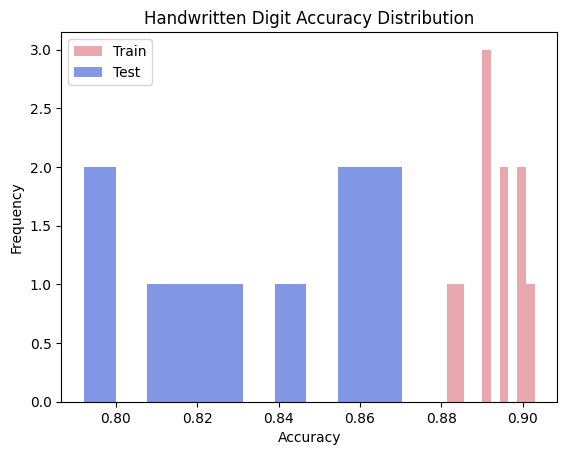
\includegraphics[width=\linewidth]{figures/digit_acc_dt.png}
        \caption{Handwritten Digits Accuracy Distribution}
    \end{minipage}\hfill % This adds horizontal space between the two
    % Second Image
    \begin{minipage}{0.48\textwidth}
        \centering
        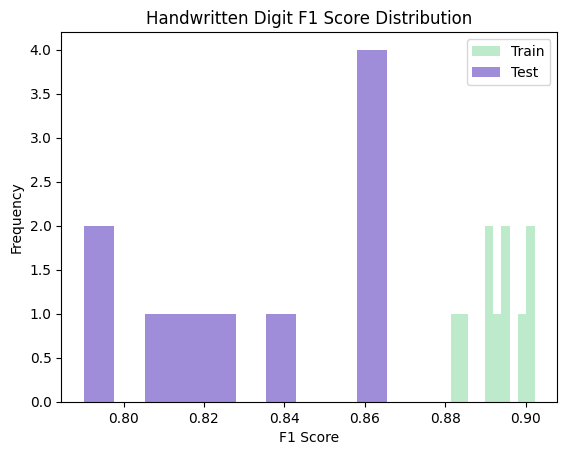
\includegraphics[width=\linewidth]{figures/digit_f1_dt.png}
        \caption{Handwritten Digits F1 Score Distribution}
    \end{minipage}
\end{figure}

Analysis about graph

\newpage 




\section{\underline{The Oxford Parkinson's Disease Detection Dataset}}

\subsection{Neural Networks Algorithm}

TODO

\noindent\rule{\textwidth}{0.5pt}

\subsection{Algorithm 2}

TODO 

\noindent\rule{\textwidth}{0.5pt}

\subsection{Decision Trees Algorithm}

\begin{verbatim}
Tuning for dataset with 195 rows and 22 features.
Testing Depths: [2, 3, 5, 7, 9, 11, 13]
Testing Splits: [9, 19, 29, 39]

Depth    | Split    | Test Acc   | Test F1   
---------------------------------------------
2        | 9        | 0.8503     | 0.8065
2        | 19       | 0.8117     | 0.7631
2        | 29       | 0.8454     | 0.7922
2        | 39       | 0.8625     | 0.7836
3        | 9        | 0.8681     | 0.8278
3        | 19       | 0.8312     | 0.7890
3        | 29       | 0.8309     | 0.7553
3        | 39       | 0.8620     | 0.7975
5        | 9        | 0.8575     | 0.8157
5        | 19       | 0.8556     | 0.8171
5        | 29       | 0.8362     | 0.7784
5        | 39       | 0.8611     | 0.7906
7        | 9        | 0.8456     | 0.8050
7        | 19       | 0.8211     | 0.7456
7        | 29       | 0.8312     | 0.7815
7        | 39       | 0.8617     | 0.7912
9        | 9        | 0.8323     | 0.7762
9        | 19       | 0.8515     | 0.8086
9        | 29       | 0.8534     | 0.8038
9        | 39       | 0.8512     | 0.7767
11       | 9        | 0.8562     | 0.7975
11       | 19       | 0.8220     | 0.7627
11       | 29       | 0.8273     | 0.7595
11       | 39       | 0.8606     | 0.7840
13       | 9        | 0.8628     | 0.8177
13       | 19       | 0.8361     | 0.7720
13       | 29       | 0.8348     | 0.7692
13       | 39       | 0.8495     | 0.7635

==============================
BEST CONFIGURATION:
Max Depth: 3
Min Split: 9
F1 Score:  0.8278
==============================


Final Results:
Training Accuracy: 0.9345
Training F1 Score: 0.9165
Testing Accuracy: 0.8508
Testing F1 Score: 0.8101
\end{verbatim}


\begin{figure}[htbp]
    \centering
    % First Image
    \begin{minipage}{0.48\textwidth}
        \centering
        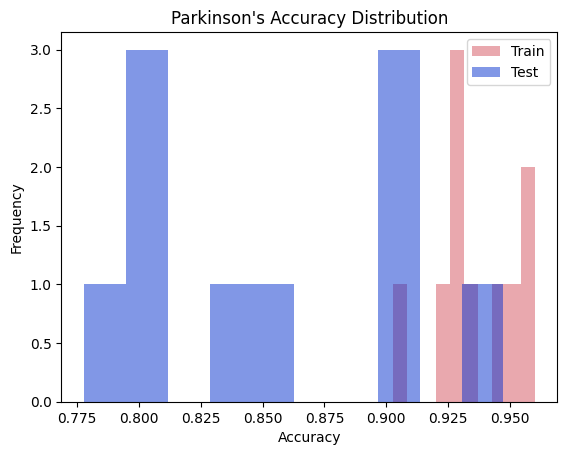
\includegraphics[width=\linewidth]{figures/park_acc_dt.png}
        \caption{Oxford Parkinson's Disease Detection Accuracy Distribution}
    \end{minipage}\hfill % This adds horizontal space between the two
    % Second Image
    \begin{minipage}{0.48\textwidth}
        \centering
        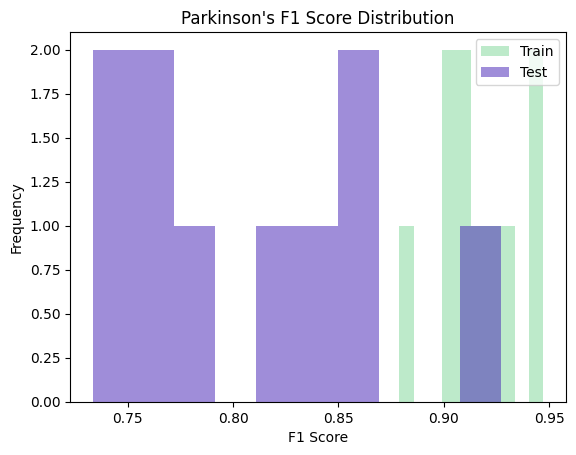
\includegraphics[width=\linewidth]{figures/park_f1_dt.png}
        \caption{Oxford Parkinson's Disease Detection F1 Score Distribution}
    \end{minipage}
\end{figure}

\newpage




\section{\underline{The Rice Grain Dataset}}
\subsection{Neural Networks Algorithm}

TODO

\noindent\rule{\textwidth}{0.5pt}

\subsection{Algorithm 2}

TODO 

\noindent\rule{\textwidth}{0.5pt}

\subsection{Decision Trees Algorithm}
We chose to test decision trees on the rice dataset 
because it has a moderate number of features (7) and a 
relatively large number of samples (3810), which allows 
us to explore how different tree depths and minimum split 
sizes affect performance.

\begin{verbatim}
Tuning for dataset with 3810 rows and 7 features.
Testing Depths: [2, 3, 5, 7, 9, 11]
Testing Splits: [190, 381, 571, 762]

Depth    | Split    | Test Acc   | Test F1   
---------------------------------------------
2        | 190      | 0.9215     | 0.9192
2        | 381      | 0.9228     | 0.9205
2        | 571      | 0.9226     | 0.9202
2        | 762      | 0.9239     | 0.9215
3        | 190      | 0.9234     | 0.9210
3        | 381      | 0.9213     | 0.9189
3        | 571      | 0.9202     | 0.9179
3        | 762      | 0.9239     | 0.9215
5        | 190      | 0.9213     | 0.9189
5        | 381      | 0.9234     | 0.9210
5        | 571      | 0.9226     | 0.9202
5        | 762      | 0.9239     | 0.9215
7        | 190      | 0.9223     | 0.9199
7        | 381      | 0.9226     | 0.9203
7        | 571      | 0.9215     | 0.9192
7        | 762      | 0.9239     | 0.9215
9        | 190      | 0.9234     | 0.9210
9        | 381      | 0.9220     | 0.9197
9        | 571      | 0.9239     | 0.9215
9        | 762      | 0.9239     | 0.9215
11       | 190      | 0.9223     | 0.9199
11       | 381      | 0.9220     | 0.9197
11       | 571      | 0.9218     | 0.9194
11       | 762      | 0.9239     | 0.9215

==============================
BEST CONFIGURATION:
Max Depth: 11
Min Split: 762
F1 Score:  0.9215
==============================



Final Results:
Training Accuracy: 0.9239
Training F1 Score: 0.9216
Testing Accuracy: 0.9239
Testing F1 Score: 0.9215
\end{verbatim}

\begin{figure}[htbp]
    \centering
    % First Image
    \begin{minipage}{0.48\textwidth}
        \centering
        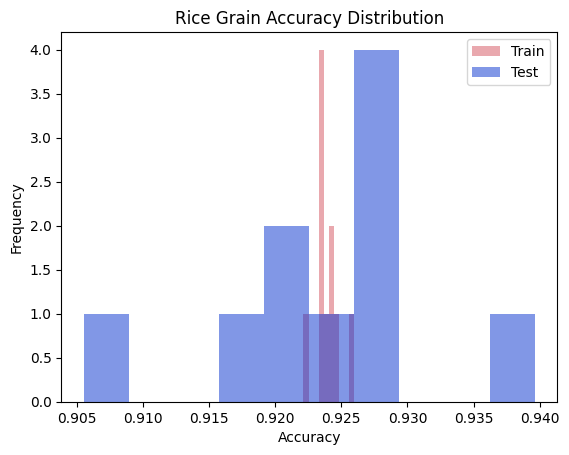
\includegraphics[width=\linewidth]{figures/rice_acc_dt.png}
        \caption{Rice Accuracy Distribution}
    \end{minipage}\hfill % This adds horizontal space between the two
    % Second Image
    \begin{minipage}{0.48\textwidth}
        \centering
        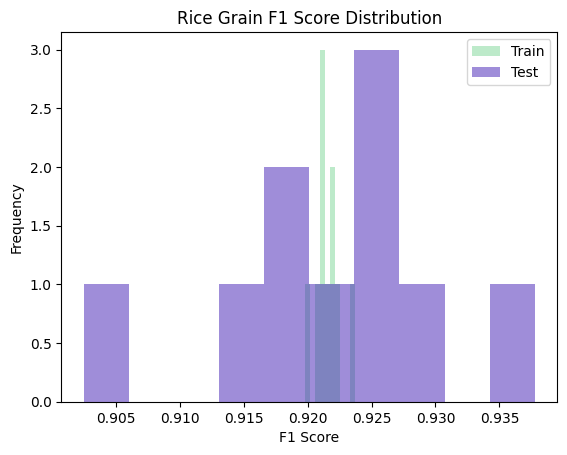
\includegraphics[width=\linewidth]{figures/rice_f1_dt.png}
        \caption{Rice F1 Score Distribution}
    \end{minipage}
\end{figure}

For both models, the training scores are highly concentrated around 0.92, 
while the testing scores are more spread out, with a mean around 0.923 for 
accuracy and 0.922 for F1 score. The training performance suggests that 
the models have high stability and low bias, however, the testing performance 
indicates that there may be some sensitivity to the specific training data used in each fold.
Since the mean training scores are very close to the mean testing scores, it suggests 
that the models are robust and are not overfitting.
Decision trees can easily split numerical features to find precise boundaries, 
so they are well-suited for the rice dataset, which consists of numerical attributes.

\newpage




\section{\underline{The Credit Approval Dataset}}
\subsection{Neural Networks Algorithm}

TODO

\noindent\rule{\textwidth}{0.5pt}

\subsection{Algorithm 2}

TODO 

\noindent\rule{\textwidth}{0.5pt}

\subsection{Decision Trees Algorithm}

\begin{verbatim}
Tuning for dataset with 653 rows and 15 features.
Testing Depths: [2, 4, 6, 8, 10, 12]
Testing Splits: [32, 65, 97, 130]

Depth    | Split    | Test Acc   | Test F1   
---------------------------------------------
2        | 32       | 0.8622     | 0.8621
2        | 65       | 0.8639     | 0.8636
2        | 97       | 0.8622     | 0.8622
2        | 130      | 0.8622     | 0.8620
4        | 32       | 0.8378     | 0.8358
4        | 65       | 0.8482     | 0.8473
4        | 97       | 0.8588     | 0.8580
4        | 130      | 0.8577     | 0.8566
6        | 32       | 0.8318     | 0.8293
6        | 65       | 0.8302     | 0.8288
6        | 97       | 0.8501     | 0.8491
6        | 130      | 0.8610     | 0.8606
8        | 32       | 0.8378     | 0.8356
8        | 65       | 0.8576     | 0.8568
8        | 97       | 0.8496     | 0.8489
8        | 130      | 0.8620     | 0.8612
10       | 32       | 0.8377     | 0.8356
10       | 65       | 0.8409     | 0.8397
10       | 97       | 0.8437     | 0.8423
10       | 130      | 0.8504     | 0.8495
12       | 32       | 0.8375     | 0.8350
12       | 65       | 0.8451     | 0.8439
12       | 97       | 0.8668     | 0.8654
12       | 130      | 0.8635     | 0.8626

==============================
BEST CONFIGURATION:
Max Depth: 12
Min Split: 97
F1 Score:  0.8654
==============================


Final Results:
Training Accuracy: 0.8746
Training F1 Score: 0.8741
Testing Accuracy: 0.8606
Testing F1 Score: 0.8601
\end{verbatim}

\begin{figure}[htbp]
    \centering
    % First Image
    \begin{minipage}{0.48\textwidth}
        \centering
        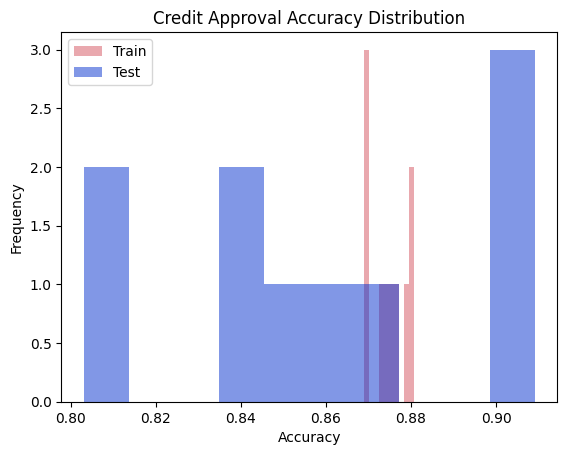
\includegraphics[width=\linewidth]{figures/credit_acc_dt.png}
        \caption{Credit Approval Accuracy Distribution}
    \end{minipage}\hfill % This adds horizontal space between the two
    % Second Image
    \begin{minipage}{0.48\textwidth}
        \centering
        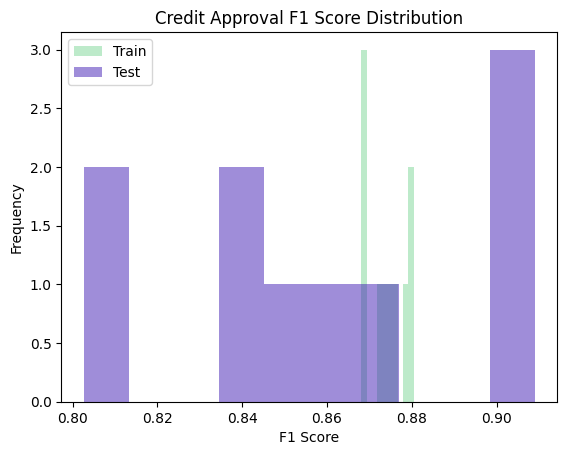
\includegraphics[width=\linewidth]{figures/credit_f1_dt.png}
        \caption{Credit Approval F1 Score Distribution}
    \end{minipage}
\end{figure}

\newpage
\begin{table}[]
\begin{tabular}{|c|cc|cc|cc|cc|}
\hline
                    & \multicolumn{2}{c|}{Handwritten Digits}  & \multicolumn{2}{c|}{Parkinson's}         & \multicolumn{2}{c|}{Rice Grains}         & \multicolumn{2}{c|}{Credit Approval}     \\ \hline
                    & \multicolumn{1}{c|}{Accuracy} & F1-Score & \multicolumn{1}{c|}{Accuracy} & F1-Score & \multicolumn{1}{c|}{Accuracy} & F1-Score & \multicolumn{1}{c|}{Accuracy} & F1-Score \\ \hline
Neural Networks     & \multicolumn{1}{c|}{}         &          & \multicolumn{1}{c|}{}         &          & \multicolumn{1}{c|}{}         &          & \multicolumn{1}{c|}{}         &          \\ \hline
K-Nearest Neighbors & \multicolumn{1}{c|}{}         &          & \multicolumn{1}{c|}{}         &          & \multicolumn{1}{c|}{}         &          & \multicolumn{1}{c|}{}         &          \\ \hline
Decision Trees      & \multicolumn{1}{c|}{0.8344}   & 0.8327   & \multicolumn{1}{c|}{0.8508}   & 0.8101   & \multicolumn{1}{c|}{0.9239}   & 0.9215   & \multicolumn{1}{c|}{0.8606}   & 0.8601   \\ \hline
\end{tabular}
\end{table}

%-------- Extra Credit Questions --------------------------
\newpage
\noindent \textcolor{purple}{\textbf{\Large{Extra Credit}}}
\vspace{0.6cm}

\noindent We did the following extra credit tasks. Describe what you did as part of that task and present the corresponding results. Any source code you develop should be included in your Gradescope submission.




    %---- Extra Credit Question QE.1 ----------------------
    \vspace{1.25cm}
    \noindent \textbf{\HIGHLIGHT{[QE.1] [Extra Credit Question \raisebox{0.2ex}{\scalebox{0.8}{\textnormal{\#}}}1]~(\POINTS{10 Points})}} 
    \vspace{0.3cm}
    
    \noindent You may earn up to 10 extra points if you analyze all four datasets using an additional algorithm. In other
words, you would be evaluating more than two algorithms on each of the datasets discussed in Section 1.

    %---- Extra Credit Question QE.2 ----------------------
    \vspace{1.25cm}
    \noindent \textbf{\HIGHLIGHT{[QE.2] [Extra Credit Question \raisebox{0.2ex}{\scalebox{0.8}{\textnormal{\#}}}2]~(\POINTS{10 Points})}} 
    \vspace{0.3cm}
    
    \noindent You may earn up to 10 extra points if you select a new challenging dataset and evaluate the performance of
different algorithms on it. A challenging dataset should necessarily include both categorical and numerical
attributes and have more than two classes; or it should be a dataset where you have to classify images.




    %---- Extra Credit Question QE.3 ----------------------
    \vspace{1.25cm}
    \noindent \textbf{\HIGHLIGHT{[QE.3] [Extra Credit Question \raisebox{0.2ex}{\scalebox{0.8}{\textnormal{\#}}}3]~(\POINTS{15 Points})}} 
    \vspace{0.3cm}
    
    \noindent You may earn up to 15 extra points if you combine different algorithms and construct an ensemble. For
instance, you could create an ensemble composed of three neural networks (each with a different architecture)
and a random forest. The ensemble would be trained as described in class: each algorithm would be trained
on its own bootstrap dataset, and so on. The final predictions would then be determined by majority voting.
Evaluate your ensemble algorithm on all four datasets discussed in Section 1.

%---- Extra Credit Question QE.4 ----------------------
    \vspace{1.25cm}
    \noindent \textbf{\HIGHLIGHT{[QE.3] [Extra Credit Question \raisebox{0.2ex}{\scalebox{0.8}{\textnormal{\#}}}3]~(\POINTS{15 Points})}} 
    \vspace{0.3cm}

    \noindent You may earn up to 15 extra points if you implement a new type of algorithm—a non-trivial variant of one
of the algorithms studied in class. If you choose to do so, you should evaluate its performance on all four
datasets.

\end{document}